\chapter{Исследовательский раздел}
В данном разделе проведен сравнительный анализ алгоритмов по используемому процессорному времени.

\section{Технические характеристики}
Технические характеристики используемого устройства:
\begin{itemize}
    \item[---] Операционная система --- Windows 10 Home \cite{Windows}
    \item[---] Память --- 16 Гб.
    \item[---] Процессор --- Intel(R) Core(TM) i5-10300H CPU @ 2.50 Ггц \cite{Intel}
    \item[---] Микроконтроллер --- STM32F303 \cite{STM}
\end{itemize}


\section{Время выполнения алгоритмов}
Время работы трех алгоритмов умножения матриц было измерено и представлено в таблице \ref{tbl:time_measurements}. Тестирование проводилось на микроконтроллере STM32F303 с тактовой частотой до 72 МГц. Измерения выполнялись на матрицах одинакового размера и усреднялись для каждого набора однотипных экспериментов. Каждое значение является средним результатом 100 замеров. График зависимости времени умножения от размера матриц для трех алгоритмов показан на рисунке \ref{fig:tm}.

\begin{table}[h]
	\begin{center}
		\begin{threeparttable}
		\captionsetup{justification=raggedright,singlelinecheck=off}
		\caption{Время работы алгоритмов (в мс)}
		\label{tbl:time_measurements}
		\begin{tabular}{|c|r|r|r|r|}
			\hline
			Размер матрицы & Классический & Виноград & Виноград (оптимизированный) \\
            \hline
			3    & 0.3 & 0.3 & 0.5 \\
            \hline
			5    & 1.1 & 1.5 & 1.3 \\ 
            \hline
			7    & 2.9 & 3.3 & 2.8 \\ 
            \hline
			9    & 5.7 & 6.4 & 5.7 \\ 
			\hline
			11    & 10.2 & 11.0 & 9.7 \\ 
			\hline
			13    & 18.0 & 18.3 & 16.3 \\ 
			\hline
			15    & 28.9 & 26.5 & 24.0 \\ 
			\hline
			17    & 39.6 & 38.6 & 36.6 \\ 
			\hline
			19    & 51.8 & 51.4 & 46.0 \\ 
			\hline
			21    & 68.7 & 72.7 & 61.9 \\ 
			\hline
			23    & 97.5 & 96.0 & 83.0 \\ 
			\hline
            25    & 122.3 & 114.1 & 108.0 \\ 
            \hline
            27    & 149.9 & 153.2 & 138.1 \\ 
            \hline
            29   & 180.1 & 175.3 & 161.8 \\ 
            \hline
            31   & 239.1 & 230.1 & 208.0 \\ 
            \hline
            33   & 282.9 & 282.9 & 247.4 \\ 
            \hline
            35   & 329.5 & 329.5 & 298.6 \\ 
            \hline
		\end{tabular}
		\end{threeparttable}
    \end{center}
\end{table}

\clearpage

\begin{figure}[H]
    \centering
    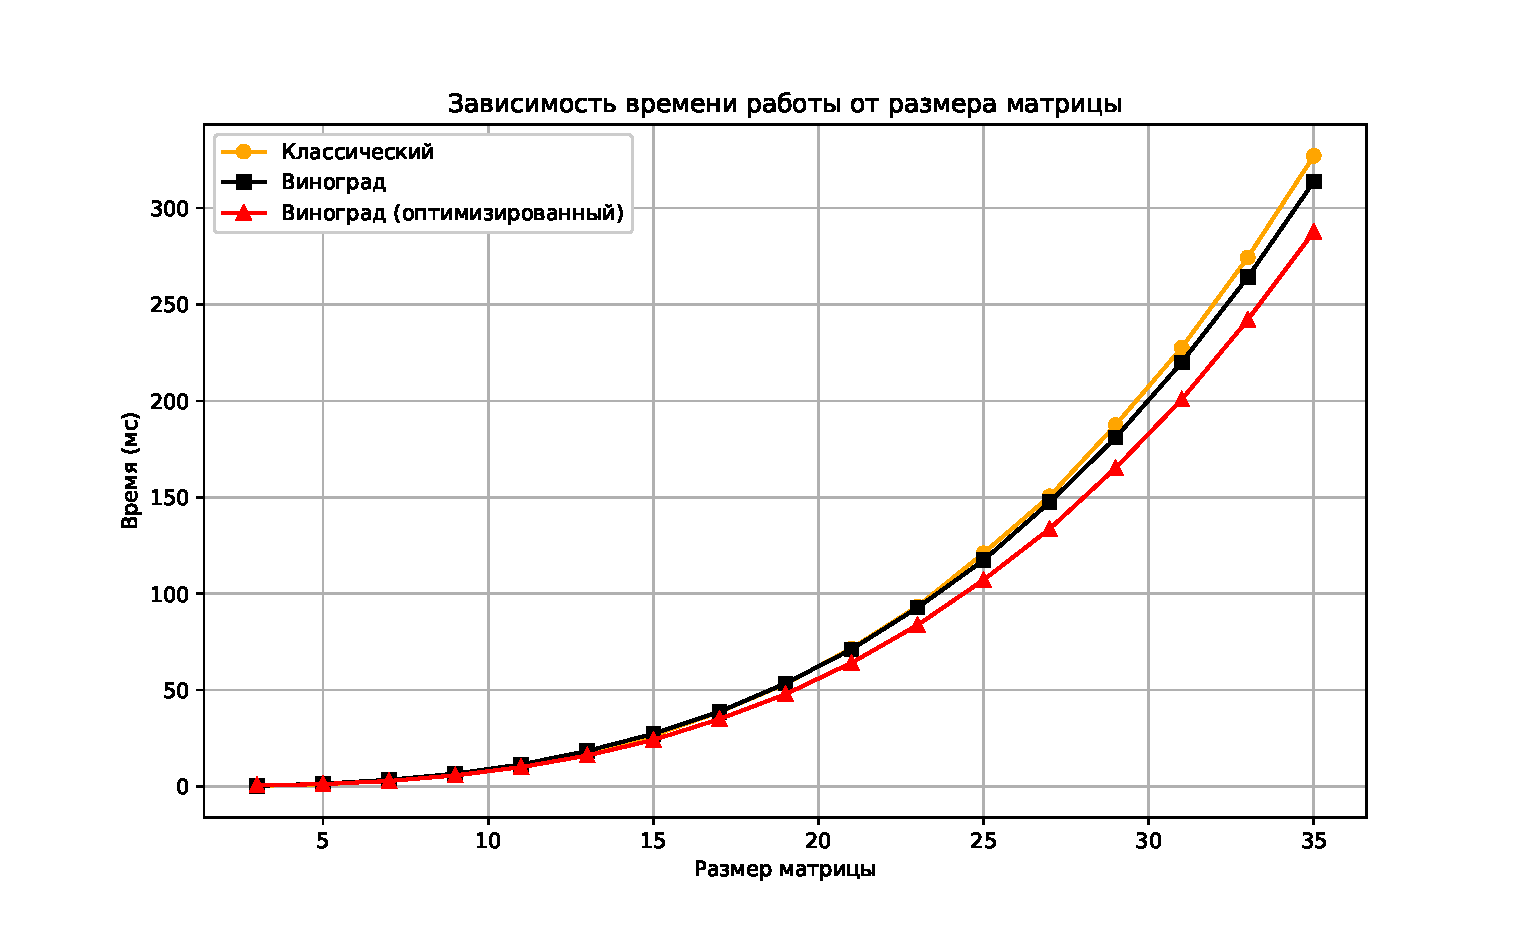
\includegraphics[width=1\linewidth]{img/graph.eps}
    \caption{Сравнение алгоритмов по времени}
    \label{fig:tm}
\end{figure}

\clearpage

\textbf{ВЫВОД}

Исследование показало, что классический алгоритм умножения матриц уступает алгоритму Винограда по скорости примерно в 1,2 раза, поскольку в алгоритме Винограда часть вычислений выполняется заранее, а количество сложных операций, таких как умножение, уменьшается. Следовательно, алгоритм Винограда предпочтительнее. Оптимизированный алгоритм Винограда, в свою очередь, демонстрирует еще лучшее время работы — он быстрее на 1,2 раза на матрицах размером более 10 элементов благодаря замене операций сложения и присваивания, сдвигу вместо умножения и предварительным вычислениям некоторых выражений. Таким образом, для наилучшей производительности стоит выбирать оптимизированный алгоритм Винограда.

Кроме того, выявлено, что на матрицах с четным размером алгоритм Винограда работает быстрее, чем на нечетных, что связано с необходимостью дополнительной обработки крайних строк и столбцов. Соответственно, алгоритм Винограда наиболее эффективен для матриц с четными размерами.